\section{Mesure sur le banc de test}
La première version du banc de test est pratique, car lors de la mise en pratique, le flux d'air pulsé est aisément vérifiable. \\
Cependant, lors des premiers tests, aucun signal n'était visible sur l'oscilloscope. Ceci peut être dû à différentes raisons :
\begin{itemize}
    \item Un mauvais contact avec les pointes ressorts
    \item La puissance du corps de chauffe n'est pas suffisante
    \item L'échantillon est défectueux
\end{itemize}

Afin de vérifier quel-s paramètre-s entraîne-nt un mauvais résultat, une première décision a été de tester le capteur ouvert (sans son support).
Des pinces plates viennent faire le contact électrique directement sur le capteur afin de mesurer la tension y circulant.
\begin{figure}[H]
    \centering
    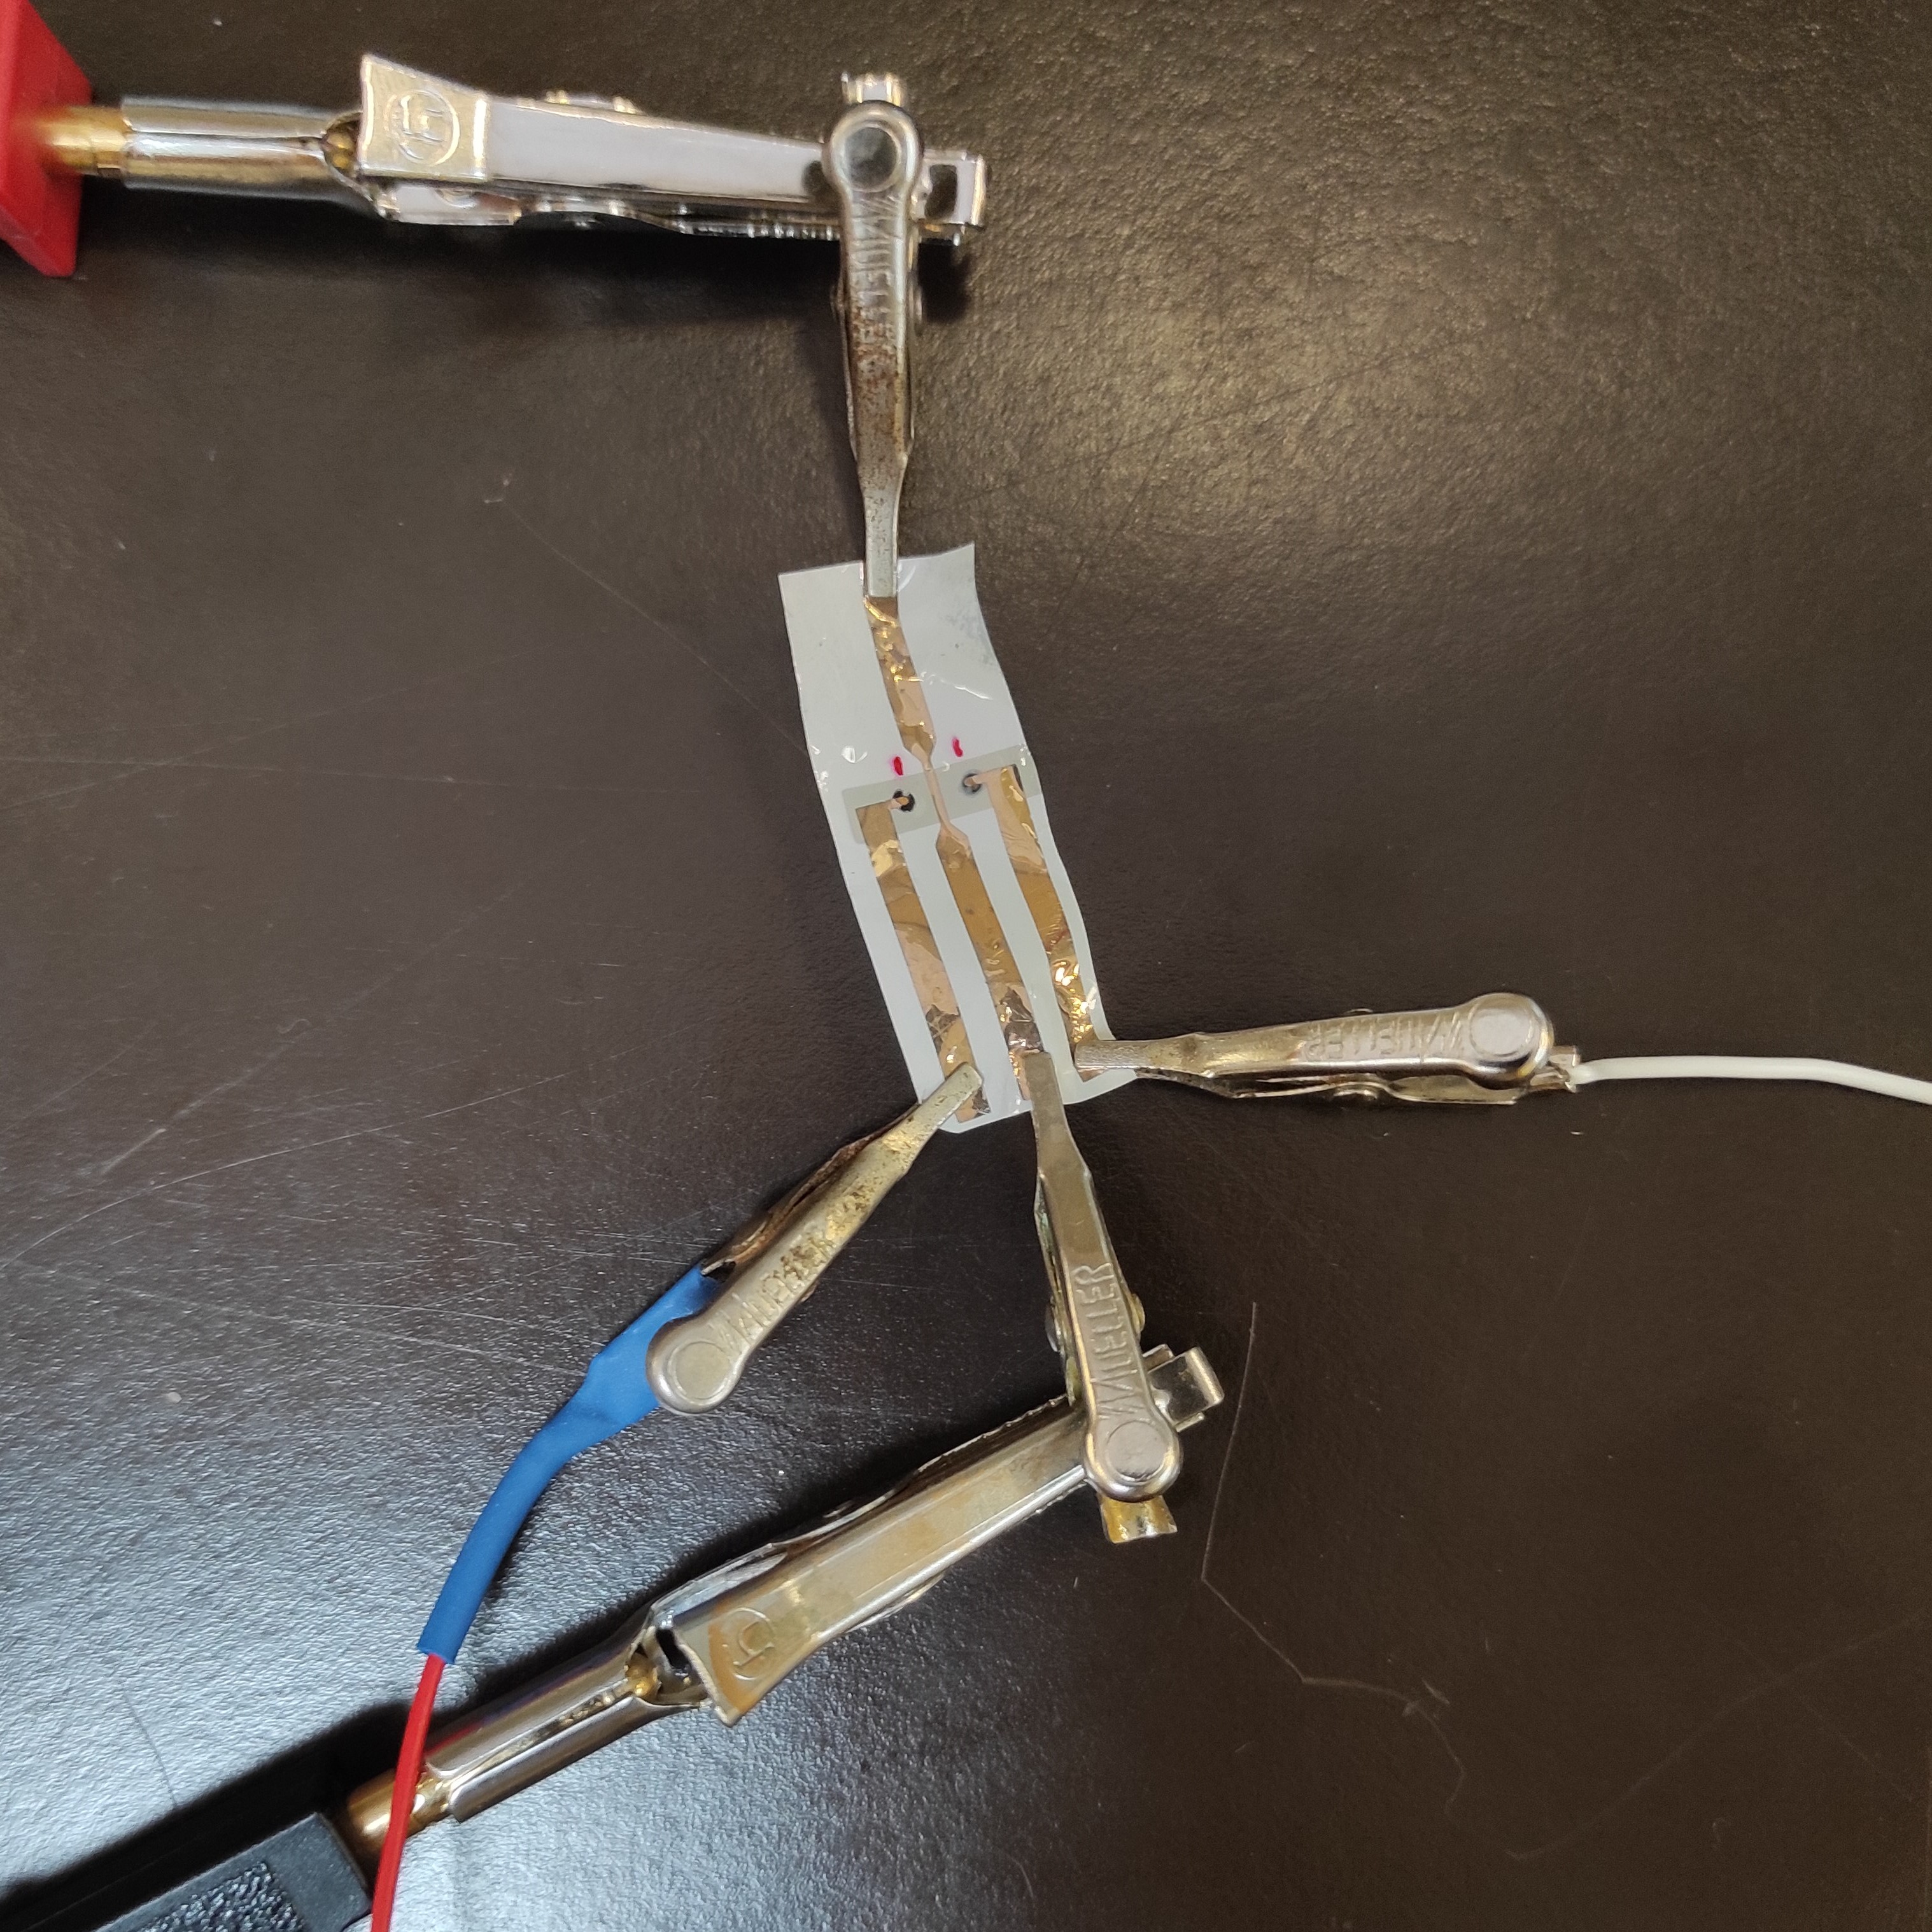
\includegraphics[scale = 0.05]{assets/figures/CapteurOuvert.jpg}
    \caption{Tests sur capteur ouvert}
    \label{fig:capteurOuvert}
\end{figure}
Cette installation ne communiquait pas non plus de résultat concluant (tension à 0V). \\

Le corps de chauffe a donc été mis en question. Une alternative à ce corps de chauffe a été de venir toucher la pince plate d'un côté du
capteur afin d'engendrer une différence de température entre les deux parties coudées. Ceci a bel et bien entraîné une différence de
température et donc, une tension. Cependant, cette dernière provient de la différence de température entre l'or (sur le capteur) et le métal
de la pince plate. \\

Afin de chauffer une des deux parties électrodéposées, une court tube a été utilisé. Un flux d'air chaud a été soufflé directement sur cette
partie afin de créer un gradient de température mais à nouveau, auncune fluctuation n'a été perçue. Cependant, lorsque le flux d'air chaud
était soufflé au niveau de la pince plate, une plus grande fluctuation de tension était visible. Cela signifie que la jonction avec le tellure
de bismuth est probablement pathologique.\\

Il était tout de même nécessaire et intéressant de vérifier si le banc de test fonctionnait de manière appropriée. Pour cela, un autre capteur
a été utilisé afin de vérifier la fonctionalité du banc de test. \\
Le capteur utilisé est un capteur infrarouge par nanotechnologie qui traduit un certain rayonnement électromagnétique en tension. Ainsi lorsque l'on souffle
dessus, un changement dans l'environnement et donc sur le rayonnement électromagnétique va se produire.
\begin{figure}[H]
    \centering
    \begin{subfigure}[b]{0.45\textwidth}
        \hspace{-1 cm}
        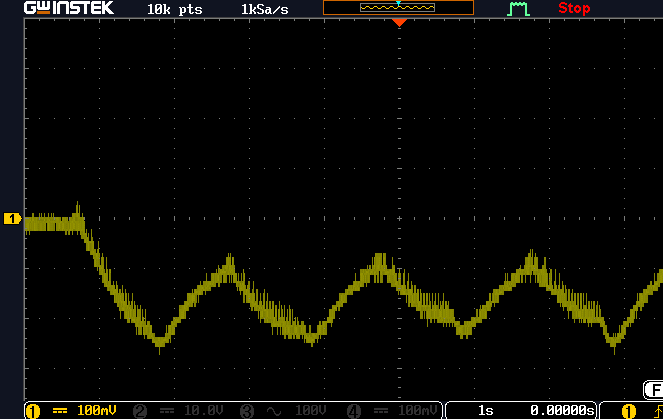
\includegraphics[scale = 0.45]{assets/figures/CapteurIR_1s_1s.PNG}
        \caption{Air pulsé pendant 1s puis repos pendant 1s}
        \label{fig:1s1s}
    \end{subfigure}
    \begin{subfigure}[b]{0.45\textwidth}
        \centering
        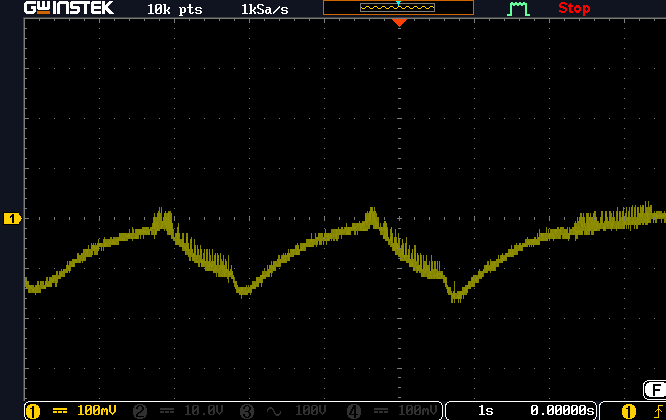
\includegraphics[scale = 0.45]{assets/figures/1_8s_repos.PNG}
        \caption{Air pulsé pendant 1s puis repos pendant 1.8s}
        \label{fig:1_8s}
    \end{subfigure}
    \caption{Résultats avec capteur infrarouge}
    \label{fig:capteurIR}
\end{figure}

Les figures ci-dessus (\ref{fig:capteurIR}), montrent que le banc de test et plus précisément, le système de flux d'air pulsé accompagné de
la sortie à l'oscilloscope (en passant par l'amplificateur) fonctionne bien. En effet, sur les figures \ref*{fig:1s1s} et \ref*{fig:1_8s}
les différentes pulsations sont bien visibles.\\

Sur la figure \ref*{fig:1s1s}, la récupération du capteur est plus longue que le temps de repos. C'est pourquoi le temps de repos a été allongé
et fixé à 1.8s (figure \ref*{fig:1_8s}). Ceci permet au capteur de se remettre à zéro et permet aussi de contrôler que la fréquence est bien
modulable. \\

Ces tests prouvent que le banc de test semble fonctionner de manière correcte. L'échantillon est alors certainement le facteur engendrant de
maunvais résultats.

Afin de pouvoir suivre tous les paramètres et le fonctionnement de notre système, une caméra thermique à également été utilisée afin d'observer
si le corps de chauffe était fonctionnel.

\section{Mesures du capteur}
\section{Dépandances}
\section{Discussion}